\chapter{Modflow radial conversion}


\textbf{Introduction} \\
The general thesis topic is pointed at the groundwater flow around a well. Due to seasonal circumstances the same well acts both as extraction and injection well. Direction of groundwater flow is alternately pointed towards and away from the well. This phenomenon can be simulated straightforward by the use of the USGS's modular hydrologic model MODFLOW. To generate adequate results in groundwater fluctuations high model accuracies are desirable, especially close to the well. The model preferably accommodates a fine-meshed grid by the implementation of a multitude of rows and columns. As a consequence model runtimes will last long. \\ However, groundwater flow around a well can (under specific conditions) be approached as a phenomenon of radial symmetry. Minor radial parameter conversions can reduce the number of dimensions in the MODFLOW model. A modification that reduces model runtimes substantially (Langevin, 2008). The section below contains a detailed description of the required radial scaling of parameters, as applied in this thesis. In addition, three examples are included to test and compare the radial scaled model performance.  
\bigskip \\
\textbf{Theoretical method} \\
MODFLOW is naturally based on rectangular geometry. Without the inclusion of specific adjustments this results in (multi layered) rectangular models. Model shapes not by definition necessary in the case of a well simulation. Under the assumption of subsurface conditions to be homogeneous and the absence of elements disturbing the regional hydraulic gradient it is possible to interpret the groundwater flow around a well as a phenomenon strictly cylindrical. Assumptions on which one would approach well flow model simulation as being axially symmetric (Figure~\ref{fig:Axially}).
\begin{figure}[h!]
 \centering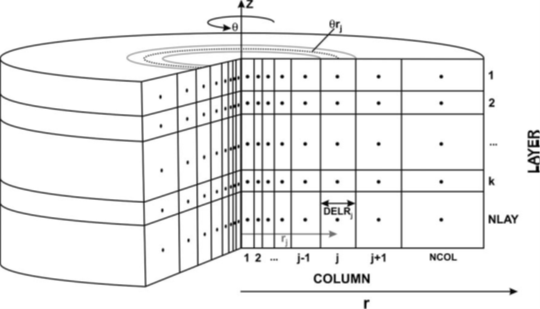
\includegraphics[width=0.5\linewidth]{Axially_symmetric}
 \captionsetup{justification=centering}
 \caption{Schematic of an axially symmetric model (Langevin, 2008)}
 \label{fig:Axially}
\end{figure} 
\bigskip \\
The in figure ~\ref{fig:Axially} displayed cylindrical approach of a well model can be simulated by an MODFLOW model (rectangular geometry) which accommodates one or more layer(s), one row only and multiple columns. In this single row model it is assumed the well is included in the first column. Moreover, the single row should act as the representation of a subsurface slice. This is achieved by the radial modification of multiple parameters. Radial parameter scaling guaranties the conversion of a rectangular (single row) MODFLOW model into a fictive radial model. Elaborating on the explanation of Langevin (2008) the following parameters become radial dependent:    
  
\begin{equation}
 K_{h}  \rightarrow K_{h,j}^{*} =  K_{h,j} \theta r_{j}
\end{equation}

\begin{equation}
 K_{v}  \rightarrow K_{v,j}^{*} = K_{v,j} \theta r_{j} 
\end{equation}

\begin{equation}
 S_{s}  \rightarrow Ss_{j}^{*} = Ss_{j} \theta r_{j} 
\end{equation}

\begin{equation}
 S_{y}  \rightarrow Sy_{j}^{*} = Sy_{j} \theta r_{j} 
\end{equation}

\begin{equation}
 n   \rightarrow n_{j}^{*} = n_{j} \theta r_{j} 
\end{equation}
\\
Where $K_h$ and $K_v$ represent the horizontal and vertical hydraulic conductivity, $S_s$ is the specific storage, $S_y$ is the specific yield (phreatic storage) and $n$ is the porosity. Scaled parameters modification is highlighted by the introduction of the superscript $^*$. As visible by the subscript $_j$ the parameters hereby become column (radial) dependent. $r_j$ is the radial distance between column $j$ and the well (column 1) and $\theta$ is the angle of the representing slice. For the purpose of radial scaling $\theta$ covers a complete ring; $\theta$== 2$\pi$.
\bigskip \\ 
Main advantage of the implementation of the radial parameter conversion is the reduction in model dimensions. At local scale (close to well) the model can contain a detailed meshed-grid without the emergence of excessive model runtimes. Moreover the parameter is applied within the common modelling program MODFLOW itself, no specialized programs are required. However, it has to be mentioned the circular model approach can only be applied under the specific assumptions of radial symmetry (Langevin, 2008).  
\bigskip \\
\textbf{Test application}\\
To validate the radial scaled model performance, a total of three fictive test exercises are applied. In these exercises a comparison is made between the radial scaled model (Figure~\ref{fig:Single row model}) and two natural rectangular based MODFLOW models \ (Figure~\ref{fig:Rectangular model} and Figure~\ref{fig:Rectangular round model}). The rectangular MODFLOW model is the most straightforward. Due to the squared shape deviations in model outcome are expected. Whereas the rectangular round MODFLOW model is manually circularized. This model accommodates the gradual increase in flow area in the radial direction. Based on Langevin (2008) it is expected the rectangular round model should approximate radial model outcomes. 
\begin{figure}[H]
	\centering
	\begin{subfigure}[b]{0.5\linewidth}
		\centering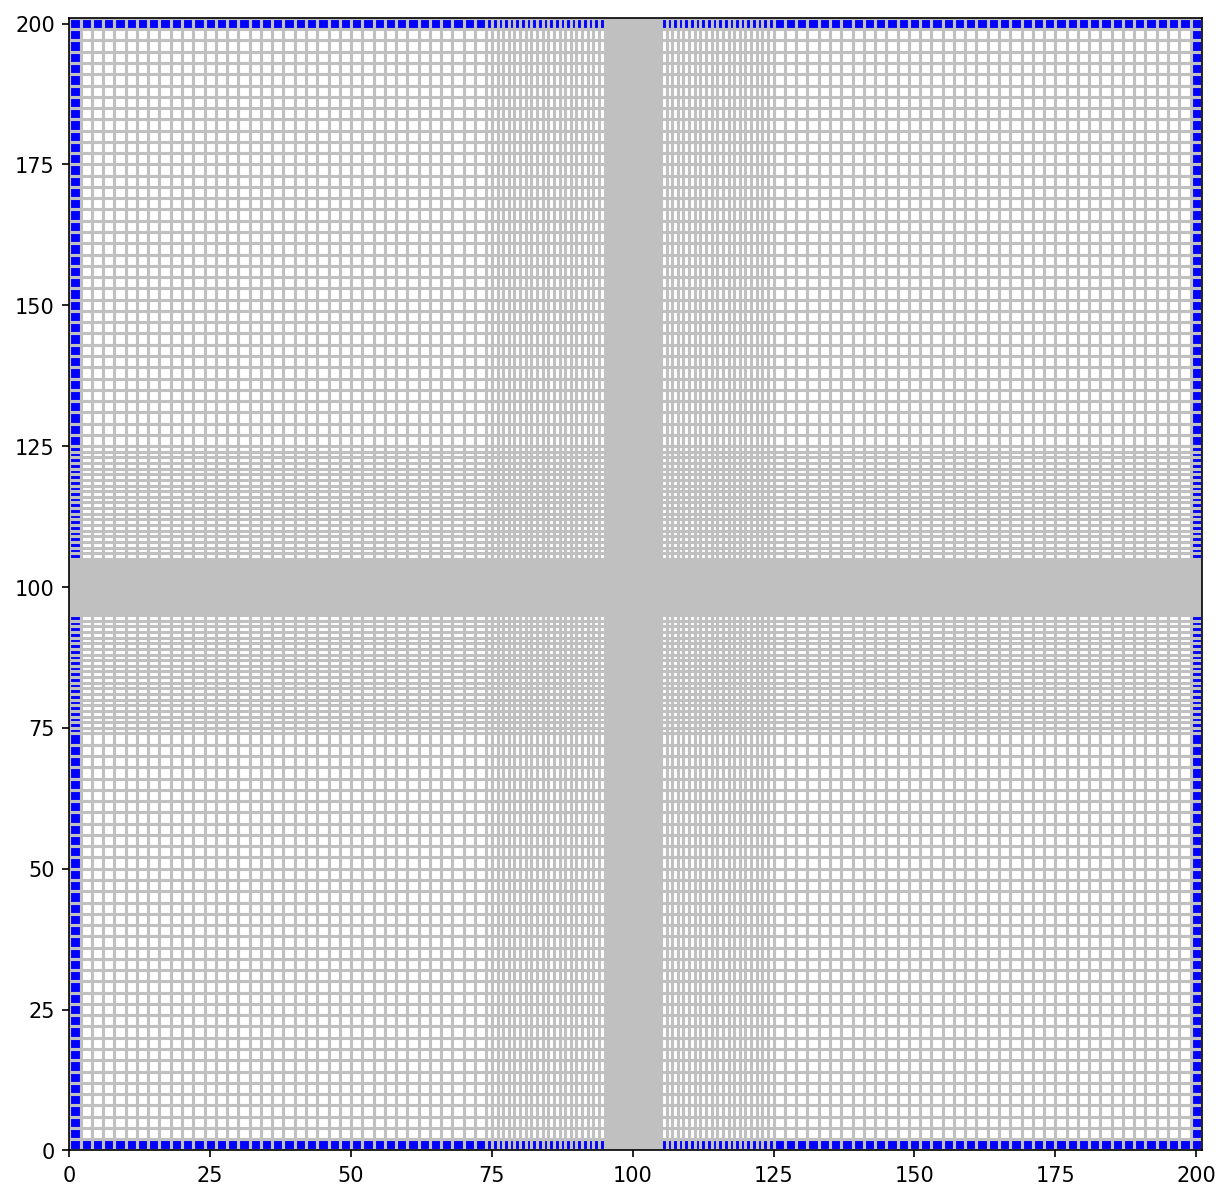
\includegraphics[width=0.9\linewidth]{Rectangular_grid}
		\captionsetup{justification=centering}		
		\caption{\label{fig:Rectangular model}}
		\end{subfigure}%\hfill
	\begin{subfigure}[b]{0.5\linewidth}
        \centering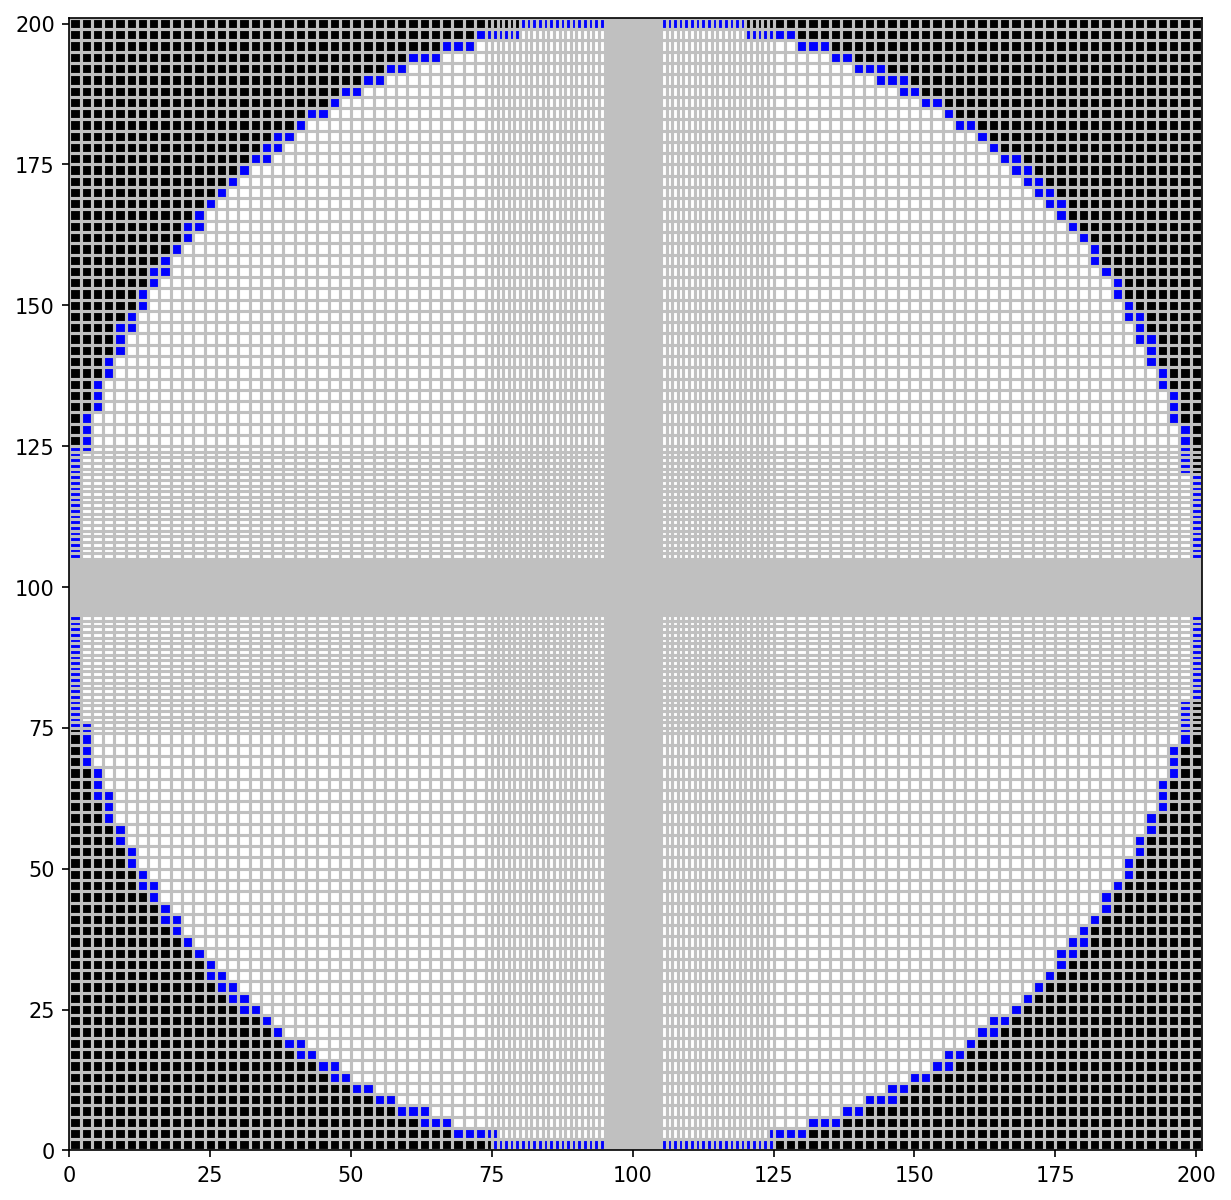
\includegraphics[width=0.9\linewidth]{Rectangular_Round_grid}
		\captionsetup{justification=centering}		
		\caption{\label{fig:Rectangular round model}}
		\end{subfigure}
	\begin{subfigure}[b]{\linewidth}
        \centering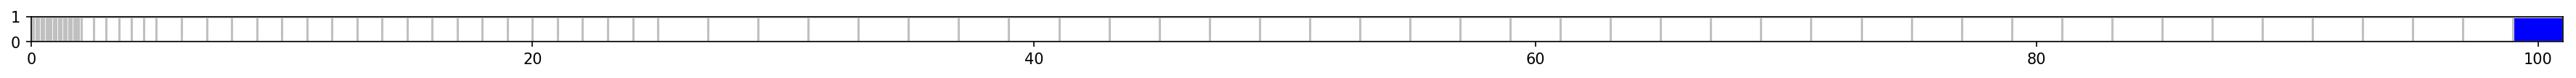
\includegraphics[width=0.95\linewidth]{Radial_grid}
		\captionsetup{justification=centering}		
		\caption{\label{fig:Single row model}}
		\end{subfigure}
	\captionsetup{justification=centering}	
	\caption[Modflow topview schematisation of a: (\subref{fig:Rectangular model}) Rectangular model, ~(\subref{fig:Rectangular round model}) Rectangular round model and ~(\subref{fig:Single row model}) Single row model]{MODFLOW topview schematisation of a: (\subref{fig:Rectangular model}) Rectangular model, ~(\subref{fig:Rectangular round model}) Rectangular round model and ~(\subref{fig:Single row model}) Single row model \\ (grey = cell boundary, red = well position, blue = boundary condition, black = inactive cell)} 
	\label{fig:Modflowtopview}
\end{figure} 
The exercises applied deliberately show strong similarities with the first two test problem cases described by Langevin (2008). In terms of content the exercises are designed with the same set of parameters, making it possible to validate the results in general. As an exception a small deviation is applied in terms of grid definition. In these exercises the cell sizes increase (grouped) stepwise based on an increasing (radial) distance from the well. By the use of the cell sizes 0.1 (20x), 0.5 (6x), 1.0 (20x) and 2.0 m (38x) a total model length (radial length) of 101 m is simulated. This grid structure is applicable on the single row (radial) model. The rectangular and rectangular round model accommodate a same and corresponding grid structure, as visible in the model top views of figure~\ref{fig:Modflowtopview}.   

\clearpage\section{Test 1: Steady flow to a fully penetrating well in confined aquifer}
\label{sec:test1}
The steady state solution of a confined aquifer fully penetrated by a well is applied as a first MODFLOW model performance test. The exercise schematic configuration is depicted in the overview of figure~\ref{fig:Schematictest1}. The case is characterized by its simplicity, making it an exercise ideally suitable for the comparison against the analytical solution. Thiem's method (Equation~\ref{eq:thiem}) is applied as the analytical drawdown solution for radial well flow in a confined aquifer (Krusseman \& de Ridder, 2000):

\begin{equation}
 S_j = \frac{Q ln(\frac{r_{2}}{r_{j}})}{2\pi K_{(h)}H}
 \label{eq:thiem}
 \end{equation} 

Where S$_j$ is the drawdown in column j, Q is the discharge, r$_2$ = 100 m (constant head at a distance of in this case 100 m from the well), $r_j$ is the radial distance between column $j$ and the well (column 1), K$_{(h)}$ is the horizontal hydraulic conductivity and H is the aquifer thickness.\\

Decline in groundwater head due to well behaviour can also be expressed directly by the use of the analytical discharge potential (strack, 1989), as depicted in (Equation~\ref{eq:potential}). Applied on confined conditions it is assumed H = h$_0$ (Source?? geo1). As a result confined heads can be determined by the application of equation \ref{eq:h_confined}. Outcomes in head are in complete correspondence with the drawdown calculated by Thiem's method. 

\begin{equation}
 \phi_j = \frac{Q}{2\pi} ln(\frac{r_j}{R}) + \phi_0
 \label{eq:potential}
\end{equation}  

\begin{equation}
 \phi_0 = k_{h}Hh_0
 \label{eq:pot_confined}
\end{equation}  

\begin{equation}
 h_j = \frac{\phi_j}{k_{h}H} 
 \label{eq:h_confined}
\end{equation}  

Where $phi_j$ is the discharge potential at column j, Q is the discharge, R = 100 m (constant head (h$_0$) at a distance of in this case 100 m from the well), $r_j$ is the radial distance between column $j$ and the well (column 1), K$_{(h)}$ is the horizontal hydraulic conductivity and H is the aquifer thickness.\\

\tikzstyle{mybox} = [draw=black, fill=white, very thick,
    rectangle, rounded corners, inner sep=30pt, inner ysep=10pt]
\tikzstyle{title} =[fill=black, text=white]

%\begin{tikzpicture}
%\node [mybox] (box){
%			\begin{minipage}{0.8\textwidth}
%			tekstje
%			\end{minipage}};    
%\end{tikzpicture}

\begin{figure}[h]
\centering
\begin{tikzpicture}
\node [mybox] (box){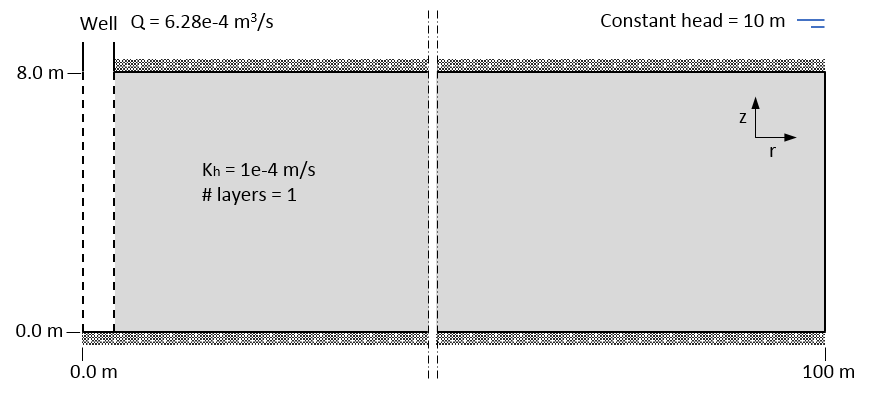
\includegraphics[width=0.6\linewidth]{Schematic_test1}};  
\node[title, right=10pt] at (box.north west) {Schematic test 1};
\end{tikzpicture}
\captionsetup{justification=centering}
\caption{Schematic test 1}
\label{fig:Schematictest1}
\end{figure}

The rectangular MODFLOW model overestimates drawdown (modelled heads are slightly lower) compared tot the analytical solution. This difference can be explained by the rectangular shape of the model; imposed boundary condition along the model edge (especially the corners) are positioned 'outside' the defined radial boundary of 100 m from the well. The rectangular round model works around this inconvenience, and already shows more similarities with the analytical solution. Some deviation in the first meter(s) around the well still exist, which can potentially be attributed to the cell structure. These minor deviations are no longer present by the application of the radial scaled (single row) model. Regardless the (radial) position, modelled heads and drawdown are identical to the analytical solution. A first indication the radial scaled MODFLOW model is preferential applicable on this thesis purposes.  

\begin{figure}[h!]
 \centering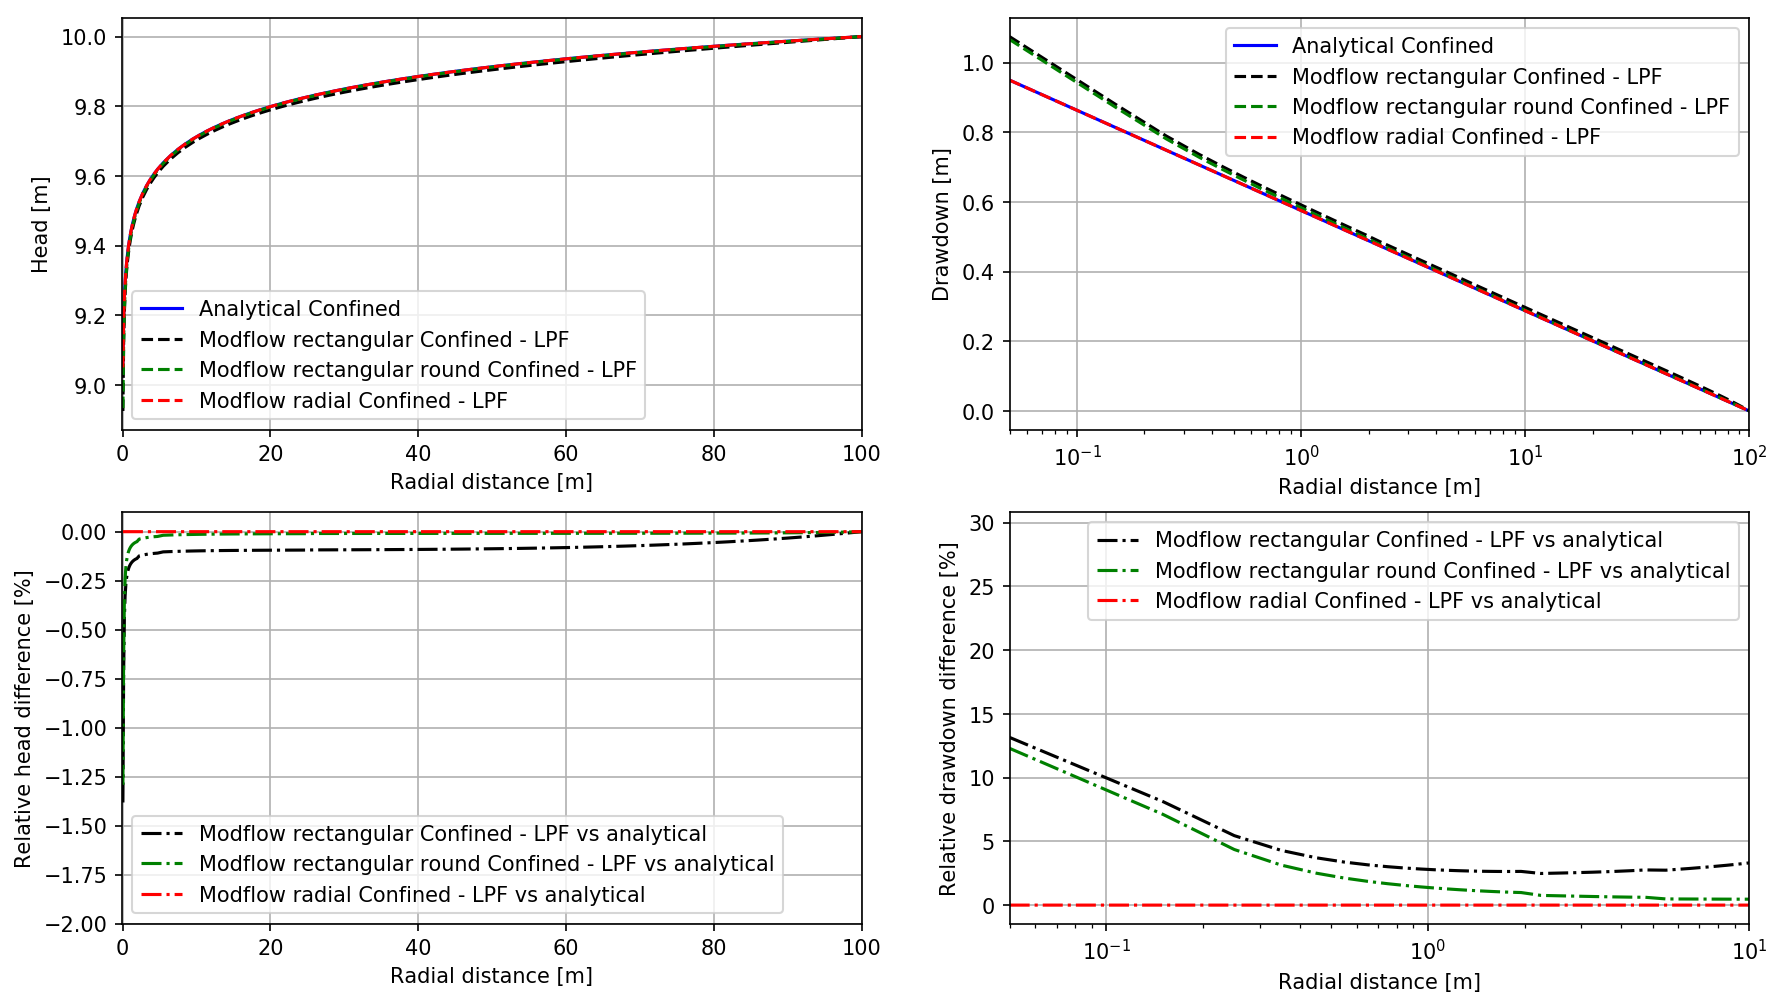
\includegraphics[width=0.8\linewidth]{Test_1_Results}
 \captionsetup{justification=centering}
 \caption{Results test 1}
 \label{fig:Test1_results}
\end{figure} 


\clearpage\section{Test 2: Steady flow to a fully penetrating well in unconfined aquifer}
Example exercise two (Figure ~\ref{fig:Schematictest2}) accommodates the same test problem as depicted in test 1, only exception is the transition towards unconfined aquifer conditions. In this example the analytical drawdown solution presented by the Thiem-Dupuit's method for steady-state flow to a fully penetrating well in an unconfined aquifer is used as a reference(Kruseman \& de Ridder, 2000):

\begin{equation}
 S'_j = \frac{Q ln(\frac{r_{2}}{r_{j}})}{2\pi K_{(h)}D}
 \label{eq:thiem_unconfined}
 \end{equation} 
 
\begin{equation}
 S'_j = S_j- \frac{S_j}{2D}  
 \label{eq:thiem_unconfined_corrected}
 \end{equation} 
 
Where S'$_j$ is the uncorrected drawdown in column j, S$_j$ is the iteratively corrected drawdown in column j, Q is the discharge, r$_2$ = 100 m (constant head at a distance of 100 m from the well), $r_j$ is the radial distance between column $j$ and the well (column 0), K$_{(h)}$ is the horizontal hydraulic conductivity and D is the thickness between aquifer bottom and constant head. For the purposes of this exercise the analytical drawdowns are iteratively determined with a precision of 1e-6. \\    

Also under unconfined conditions the analytical discharge potential (Equation~\ref{eq:potential2}) can be applied (Strack, 1989). Only exception, compared to the confined conditions, is the minor change in head derivation, visualised in \ref{eq:h_unconfined}. Major advantage, with respect to the analytical Thiem-Dupuit's method, is the absence of the iterative head derivation process. Result is the analytical calculation of even more accurate heads by the application of the discharge potential. 

\begin{equation}
 \phi_j = \frac{Q}{2\pi} ln(\frac{r_j}{R}) + \phi_0
 \label{eq:potential2}
\end{equation}  

\begin{equation}
 \phi_0 = \frac{1}{2}k_{h}h_0^{2}
 \label{eq:pot_unconfined}
\end{equation}  
 
\begin{equation}
 h_j = \sqrt{\frac{2\phi_j}{k_{h}}}
 \label{eq:h_unconfined}
\end{equation}  

Where $phi_j$ is the discharge potential at column j, Q is the discharge, R = 100 m (constant head (h$_0$) at a distance of in this case 100 m from the well), $r_j$ is the radial distance between column $j$ and the well (column 1), K$_{(h)}$ is the horizontal hydraulic conductivity and H is the aquifer thickness.\\

\begin{figure}[h]
\centering
\begin{tikzpicture}
\node [mybox] (box){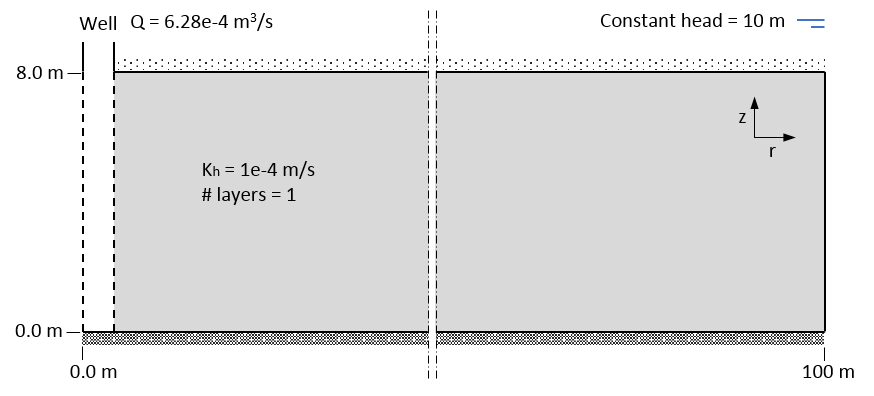
\includegraphics[width=0.6\linewidth]{Schematic_test2}};  
\node[title, right=10pt] at (box.north west) {Schematic test 2};
\end{tikzpicture}
\captionsetup{justification=centering}
\caption{Schematic test 2}
\label{fig:Schematictest2}
\end{figure}

Due to a 10 m constant head boundary the aquifer area of flow is fictive enlarged in the unconfined case (compared to the 8 m aquifer height under confined conditions). In accordance with the solutions in Langevin (2008) overall drawdowns in the unconfined conditions are slightly lower with respect to the confined situation. 
\bigskip
Model performances of the unconfined example exercise show similar behaviour as the confined example exercise. Differences in modelled and analytical determined heads and drawdowns are minuscule in general. As expected largest deviations from the analytical solution are present in the MODFLOW rectangular model. The differences in outcome of this model do persist over almost the entire radial distance from the well, regardless the use of the BCF or LPF package. Although it is only slightly, the use of the LPF package shows slightly better performance. For the purposes of this thesis the LPF package is assumed to be preferential in setting the aquifer properties. Application of this package in the MODFLOW round rectangular model results in improved model results, however deviations do continue to exist. In contract with the confined exercise (~\ref{sec:test1}) application of the radial scaled MODFLOW model under unconfined aquifer conditions  deviations from the analytical solution are still present. Modelled drawdowns show strong similarities with the uncorrected analytical solution. Moreover, relative to the analytical solution the absolute radial scaled MODFLOW model outcomes performs most accurately. Making the radial scaled (single row) MODFLOW model suitable for the unconfined aquifer conditions of this thesis.   

\begin{figure}[H]
 \centering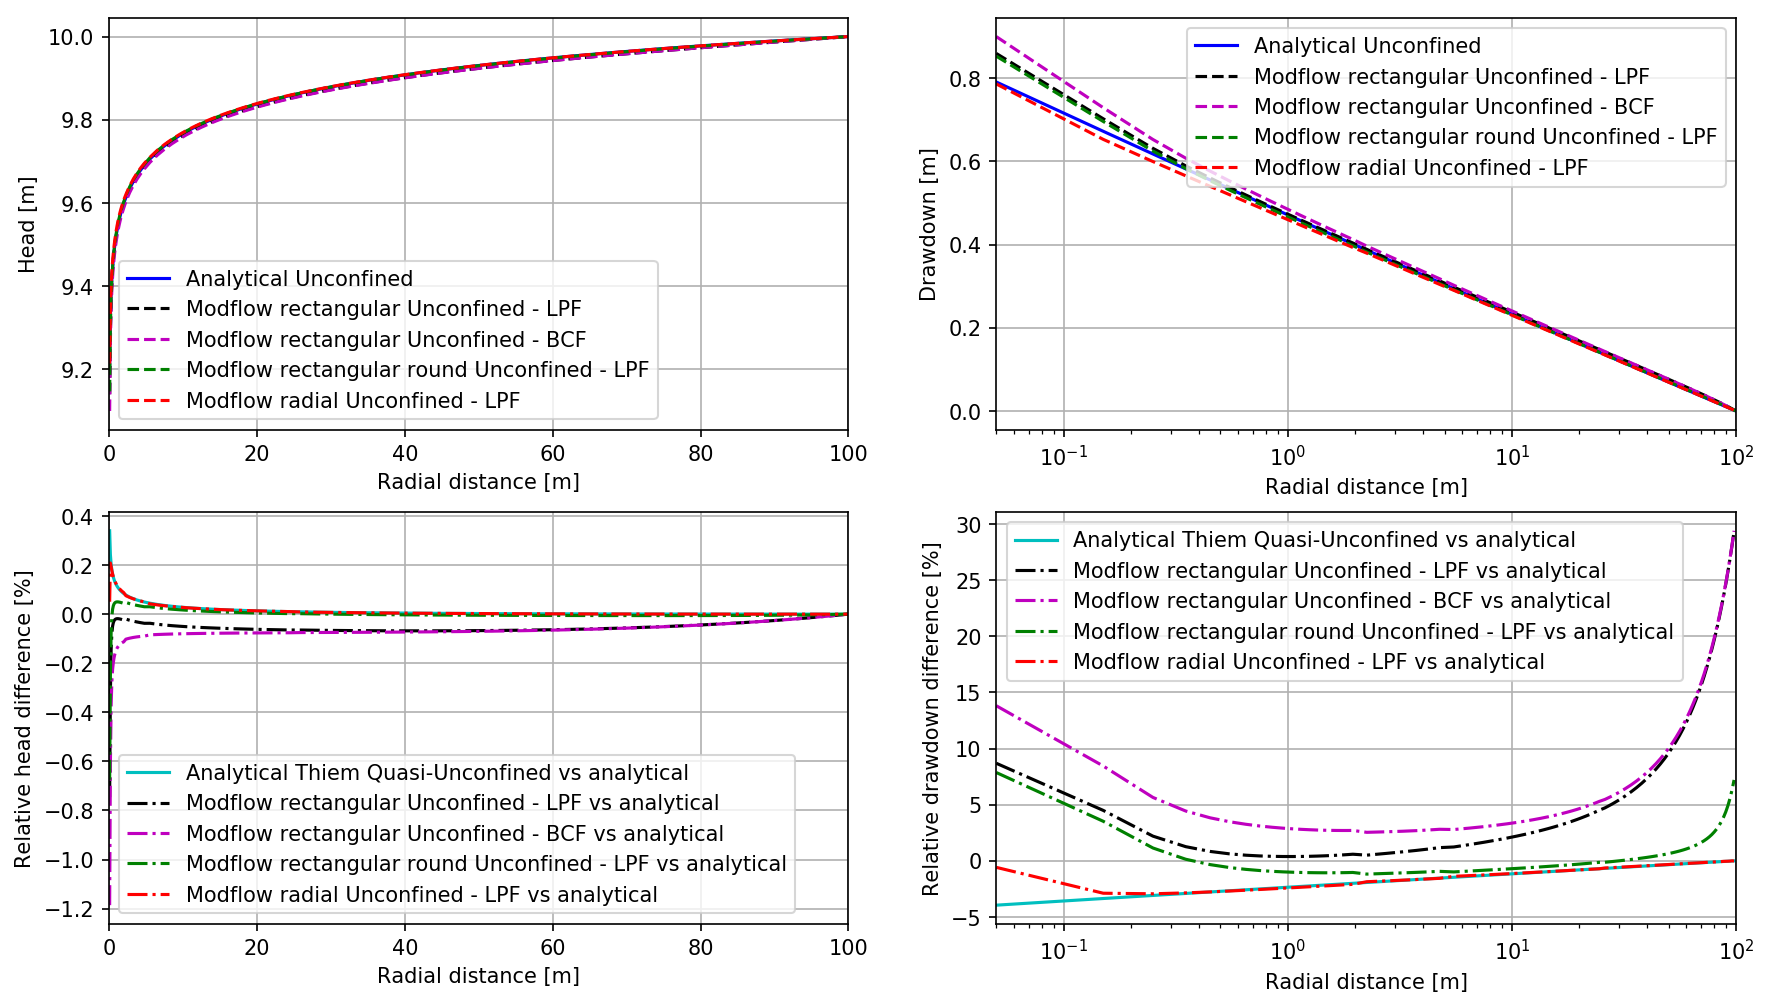
\includegraphics[width=0.8\linewidth]{Test_2_Results}
 \captionsetup{justification=centering}
 \caption{Results test 2}
 \label{fig:Test2_results}
\end{figure} 

\clearpage\section{Test 3: Unsteady flow to a partially penetrating well in unconfined aquifer}

As a final exercise the different MODFLOW models are subjected to a more complicated case (Figure ~\ref{fig:Schematictest3}). This specific exercise includes all model parameters dependent on radial scaling to test the overall radial model performance. This case accommodates a well which is partially penetrating the aquifer, making it a multi-layered problem. Sum up of the fractional discharges of the penetrating layers (48-72) results in the total well discharge. Moreover the exercise is time dependent. In this case all results are obtained after one day of groundwater withdrawal. 

\begin{figure}[h]
\centering
\begin{tikzpicture}
\node [mybox] (box){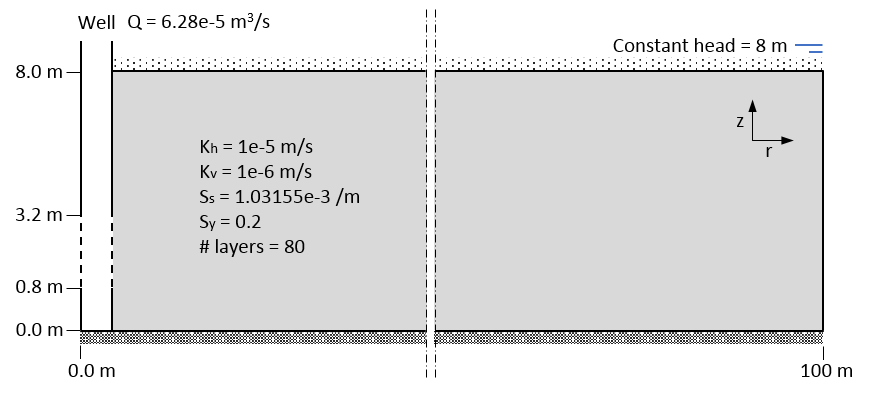
\includegraphics[width=0.6\linewidth]{Schematic_test3}};  
\node[title, right=10pt] at (box.north west) {Schematic test 3};
\end{tikzpicture}
\captionsetup{justification=centering}
\caption{Schematic test 3}
\label{fig:Schematictest3}
\end{figure}

Performance of the radial scaled (single row) MODFLOW model is visualized by the head contour plot in figure ~\ref{fig:Test3_results_contour}. From the perspective of proper comparison results of the different models are in this case shown at an height of 2.0 m (relative to aquifer bottom) along the entire aquifer (Figure ~\ref{fig:Test3.1_results}). Outcome of the comparative study is a scaled (single row) radial model which performs as expected. With the exception of the first meter(s) around the well differences between the rectangular round and the radial MODFLOW models are negligible small. Deviations at close range to the well can be attributed to the chosen grid structure. Based on the test exercises 1 and 2 it can be assumed the results of the radial model simulates the natural well behaviour properly. Application of the radial scaled (single row) MODFLOW model with the use of the LPF package is a relative fast and suitable model for this thesis purposes.  

\begin{figure}[h]
 \centering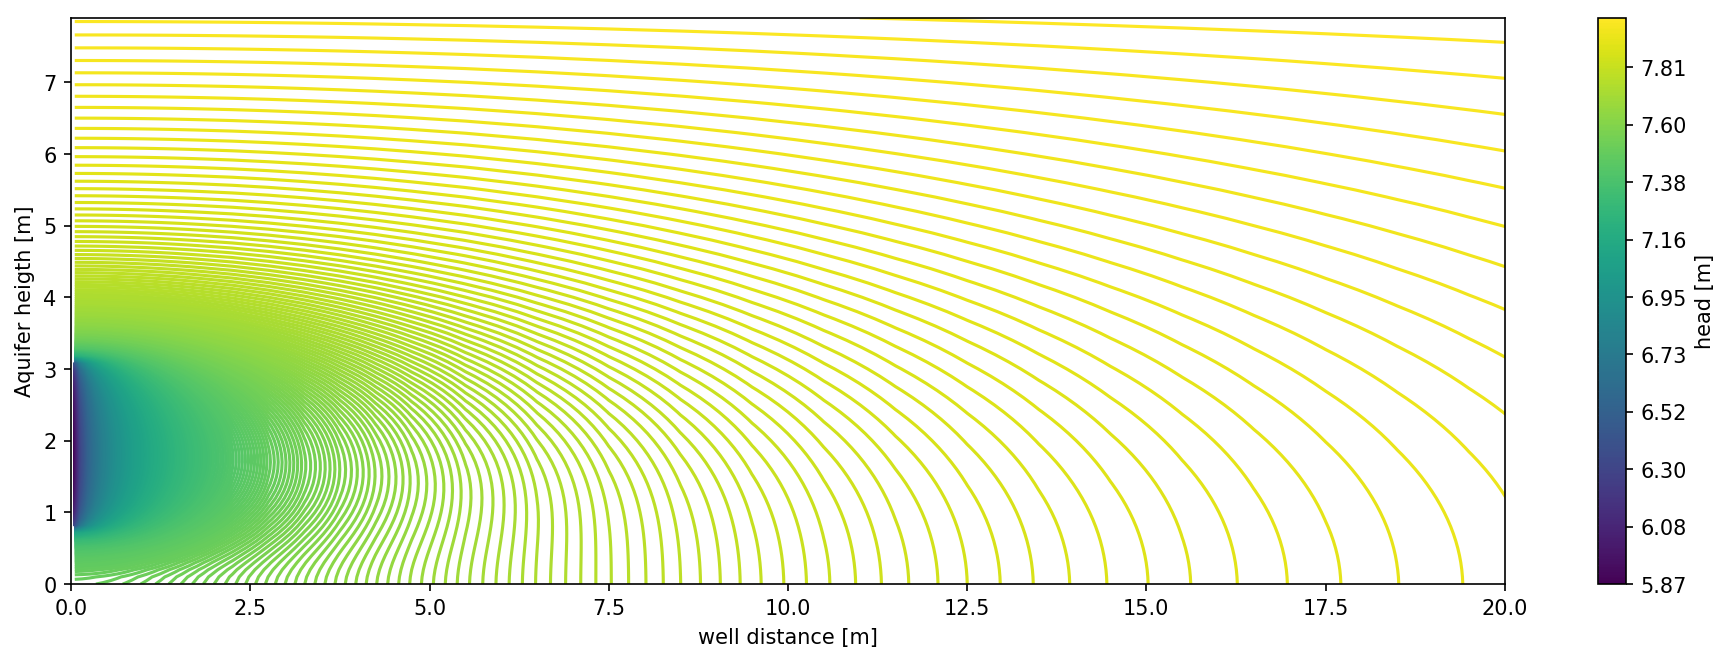
\includegraphics[width=0.8\linewidth]{Test_3_Results_contour}
 \captionsetup{justification=centering}
 \caption{Results test 3: Cross-section head contour after 1 day of pumping}
 \label{fig:Test3_results_contour}
\end{figure} 

\begin{figure}[H]
 \centering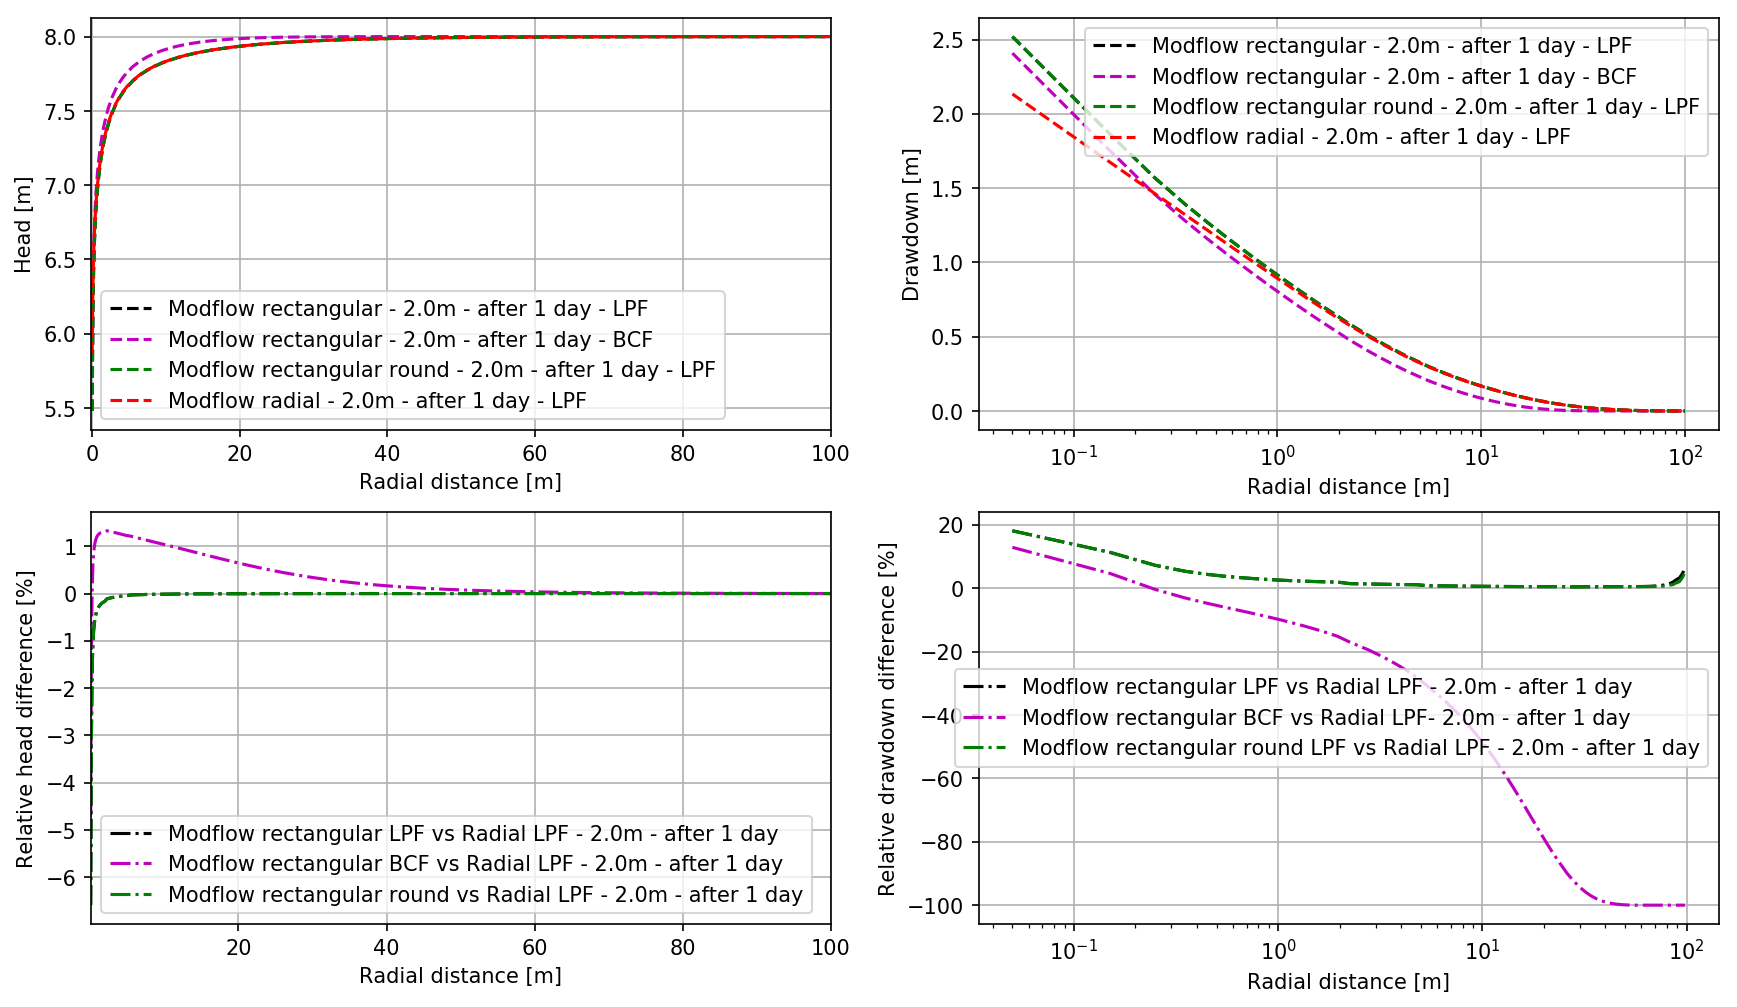
\includegraphics[width=0.8\linewidth]{Test_3_Results_2m}
 \captionsetup{justification=centering}
 \caption{Results test 3: Head after 1 day of pumping at 2.0m (relative to aquifer bottom)}
 \label{fig:Test3.1_results}
\end{figure} 
%
%\begin{figure}[h]
% \centering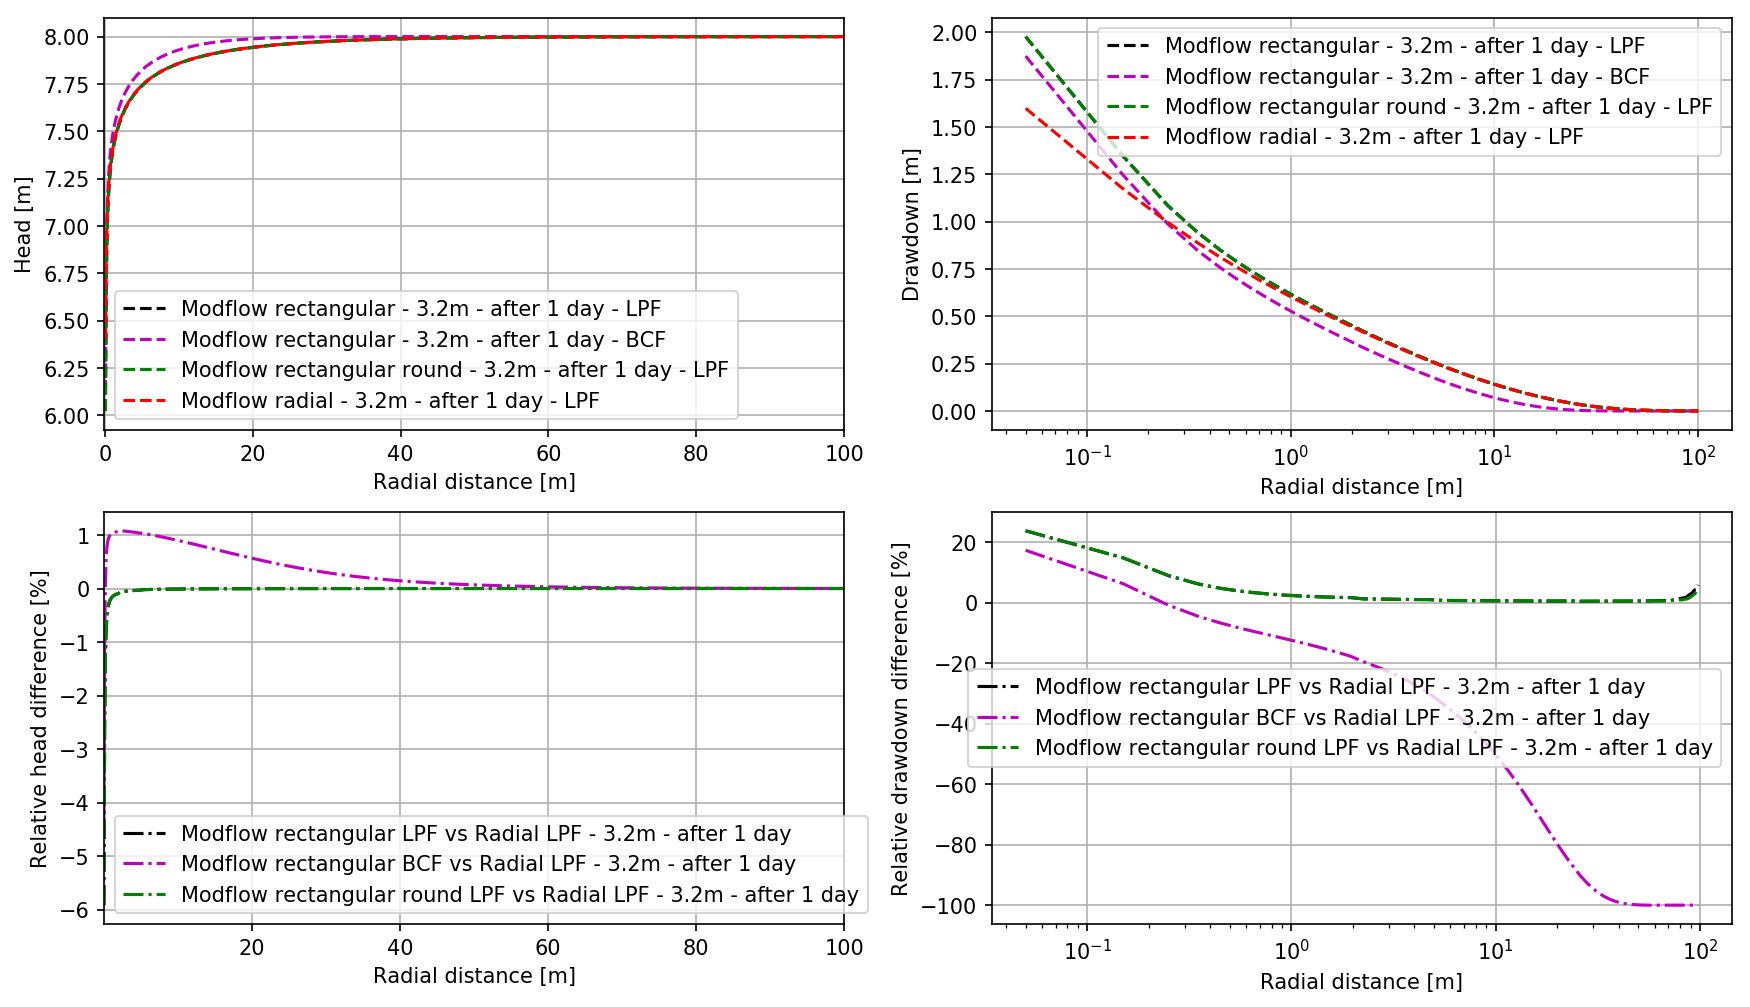
\includegraphics[width=0.8\linewidth]{Test_3_Results_3,2m}
% \captionsetup{justification=centering}
% \caption{Results test 3: at 3.2 m  (relative to bottom)}
% \label{fig:Test3.2_results}
%\end{figure} 
